\section{Week 10 - Message passing}


%The message passing scheme implemented in this task is rendezvous.

%\begin{itemize}
    %\item  What might be the motivation behind this design?
    %\item Are there any drawbacks?
    
%Processes in an operating system should be isolated from each other to prevent one badly written or malicious process from destabilizing the whole system. Any process can communicate on a port as long as it knows its index.
    
    %\item Briefly outline a scheme in which each process is given private port identifiers, i.e., identifiers or handles which can only be used by the process that obtained them.
%\end{itemize}

\textbf{Rendezvous}

Using a rendezvous scheme for message passing, means that synchronous message passing can be implemented in a simple manner. 

For rendezvous, no buffer is needed, as the message/data is injected directly from one process' address space into the other. This means, that both processes are synchronized during the data transfer. The process sending the message will therefore be blocked until the receiving process is ready, vice versa if the receiving process calls before the sending process.

Since the processes are synchronized when a message is transferred, deadlocks may occur. Two processes trying to receive a message will halt the system. This is not optimal, but a direct consequence from the rendezvous scheme. Likewise a deadlock could occur if both processes were waiting to receive a message.


\textbf{Message passing with private process identifiers}

This question can be interpreted in two ways:
\begin{enumerate}
    \item Processes can be given identifiers to other processes' ports but the identifiers are not globally available.
    \item No process can obtain the identifier of another process' port identifiers.
\end{enumerate}

\underline{For the first scenario:}

If the message passing between processes is limited to the identifiers obtained for each process, the possible channels can be written as a graph, where there are not edges between all vertices. This would lead way for specific protocols, as the messages had to follow the structure defined in the graph (dictated by the obtained interprocess port identifiers). If the \texttt{receive} command is implemented as in the labs, the edges in the graph would be bidirectional, as the receiver would obtain the identifier for the sending process in the \texttt{sender} parameter and if the port identity is known/follows a known pattern, e.g. 0 and incrementing.

\begin{figure}
    \centering
    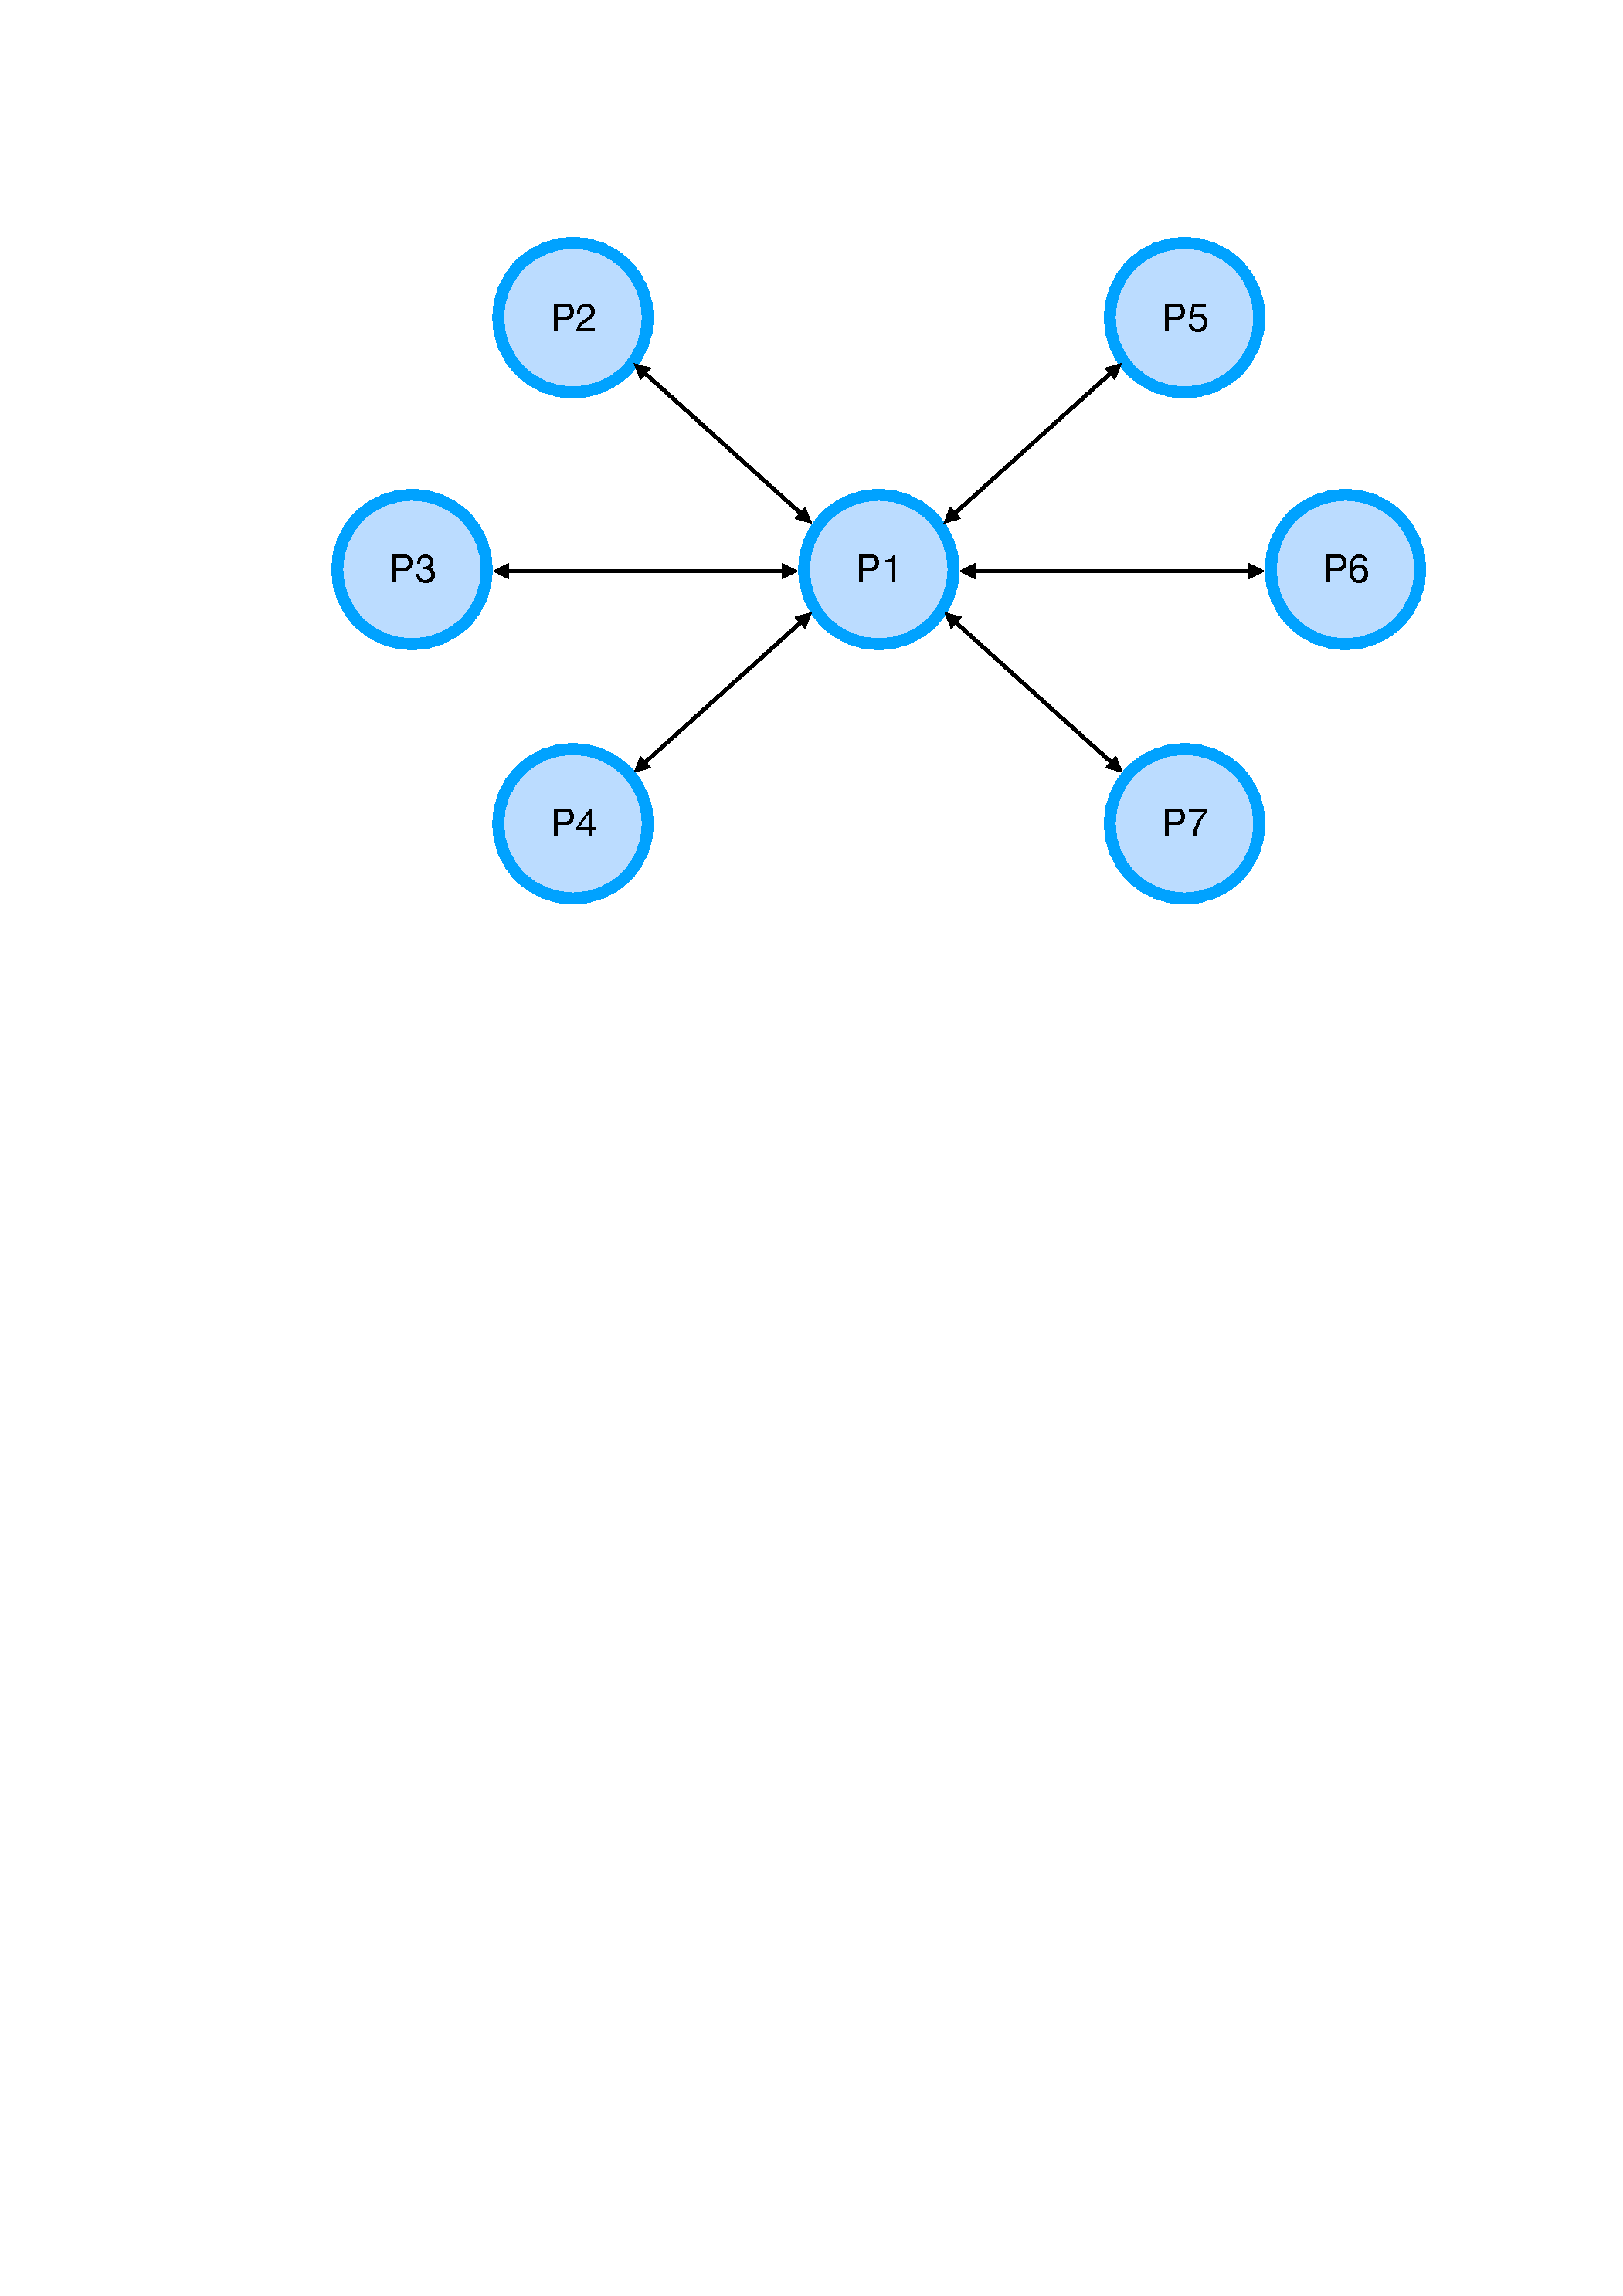
\includegraphics[width=0.7\linewidth]{fig/processGraph.pdf}
    \caption{A graph describing possible channels for message passing between processes with private port identifiers, following scenario 1. The example shows a conductor able to synchronize several processes which are not allowed/able to share information between themselves.}
    \label{fig:conductorGraph}
\end{figure}

This would be efficient if several users were using the same system, and were not allowed any form of interaction, of if several processes needed a conductor but are not allowed to share information between them. Such as graph can be seen in figure \ref{fig:conductorGraph}.

\underline{For the second scenario:}

Restricting process port information to the process itself would result in only threads from that process being able to send and receive messages between them. No two processes would be able to send/receive messages between them, and the message passing concept is therefore unnecessary, as the information and synchronization could be implemented using semaphores with shared variables, or a monitor if available in the language. With that said, the interthread message passing might lead to simpler solutions and higher performance, although it would mean a process should send messages to it's own port, meaning this should be supported by the system.

\textbf{Lab implementation of rendezvous message passing}

The message passing is implemented through the system calls; \texttt{findport}, \texttt{send} and \texttt{receive}. 

The system call for finding a port takes a port identifier and a process identity as parameters. These values correspond to the \texttt{id} of the port inside the process, and the index of the process in the process array. The ports are searched through to find a match. If a match is found, the identity for the port is returned. If no match is found, \texttt{ERROR} is returned.

When sending/receiving, one of two scenarios happens: either there is a corresponding process anticipating a receive/send in which case the rendezvous can occur, otherwise that thread of the process is blocked until further notice. Blocking threads in this case, is managed through two port pointers called \texttt{sending} and \texttt{receiving}. These pointers inform the scheduler if they are currently anticipating a send/receive (by not being null) and contain information as to what port it is waiting for, when the opposing process participates in the rendezvous. The system calls for sending and receiving are very similar; first the corresponding port pointer is set by the specified port handler given as a parameter in the \texttt{edi} register, the \texttt{sending} pointer for \texttt{send} and \texttt{receiving} for \texttt{receive}. The threads are then searched through for a match, equivalent to a thread who is anticipating the rendezvous on the same port, if a match is found the message is transferred between the two processes' address spaces.

The information contained in the message sent, is copied into the declared variable pointed to by the parameter specified on the \texttt{esi} register, meaning that the processes' address spaces never overlap, information is only send from one address space to another during the system call.

When the rendezvous has occurred their port pointers sending and receiving is set to null telling the scheduler that they are no longer blocked.

If no match was found, which would be the case for the initial \texttt{send}/\texttt{receive} call, the thread's port pointer is still set to the specified value and is set to yield, resulting in a block until the rendezvous can proceed.
